
\section{Decodificación de stream de datos en Simulink}
Se diseñó un sistema que permite realizar la decodificación de datos utilizando bloques de Simulink. Este sistema se ha probado con señales senoidales y con las señales test que tiene el mismo ADS y se ha observado que la decodificación se realiza de forma eficaz, ya que no se han observado cambios en la morfología de las señales ni en los valores de esta. El sistema diseñado se muestra en la Figura \ref{Figura: Decodi}

\begin{figure}[htbp]
	\centering
	\begin{subfigure}[htbp]{0.7\textwidth}
		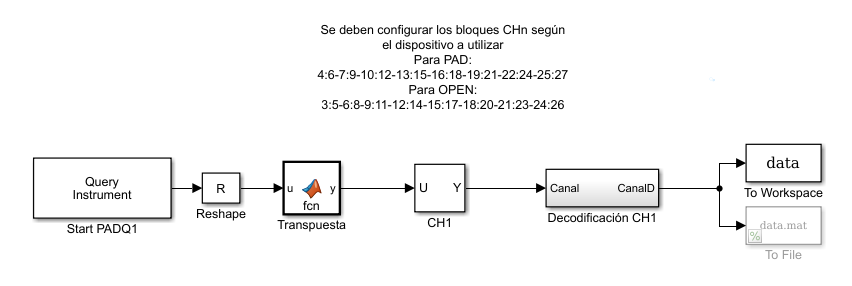
\includegraphics[width=\textwidth]{Read_Simu.png}
		\caption{Vista general del sistema diseñado para realizar la decodificación del stream de datos}
		\label{Figura: readSimu}
	\end{subfigure}
	\begin{subfigure}[htbp]{0.7\textwidth}
		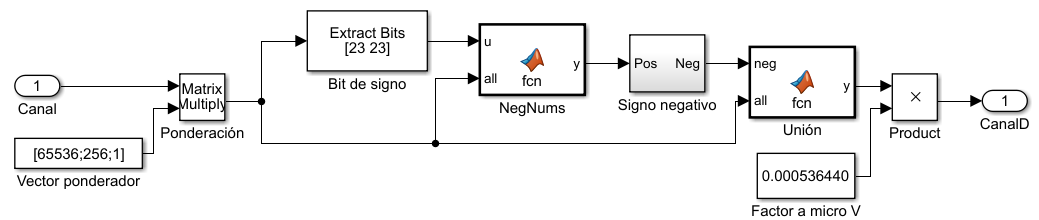
\includegraphics[width=\textwidth]{Deco_Simu.png}
		\caption{Vista interna del subsistema encargado de la decodificación de número negativos y positivos}
		\label{Figura: decoSimu}
	\end{subfigure}
	\caption{Sistema decodificador de stream de datos implementado en Simulink}
	\label{Figura: Decodi}
\end{figure}

\section{Evaluación del protocolo de comunicación para prototipo de adquisición}
Por el momento lo que se tiene son las señales sintéticas generadas en MATLAB, estas señales constan de senoidales con frecuencias de 1Hz, 5Hz, 10Hz, 20Hz y 50Hz, y también se crearon señales que representaran la fatiga del músculo, estas se crearon modulando la senoidal de 50Hz para que tuviera una atenuación lineal y una atenuación exponencial. Por último se diseñó una señal que simula el incremento de actividad de sEMG y su fatiga. Estas señales diseñadas se ilustran en la Figura \ref{Figura: SenalesEva}.

\begin{figure}[htbp]
	\centering
	\begin{subfigure}[htbp]{0.4\textwidth}
		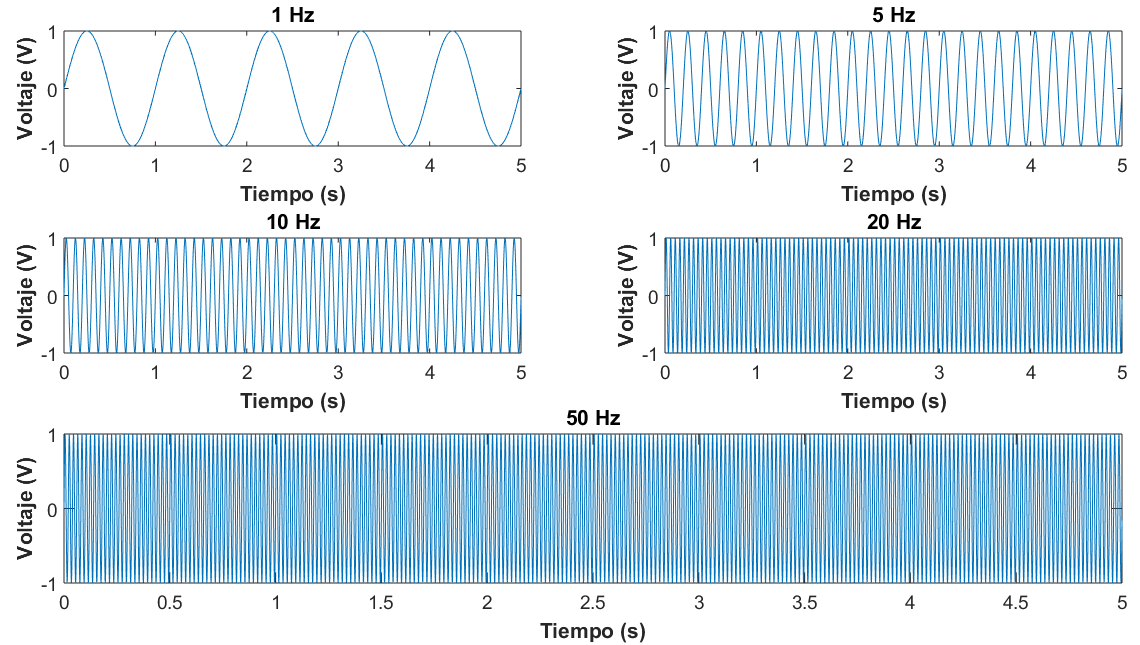
\includegraphics[width=\textwidth]{Sen_Pur.png}
		\caption{Senoidales puras a diferentes frecuencias}
		\label{Figura: SenPur}
	\end{subfigure}
	\hfill
	\begin{subfigure}[htbp]{0.4\textwidth}
		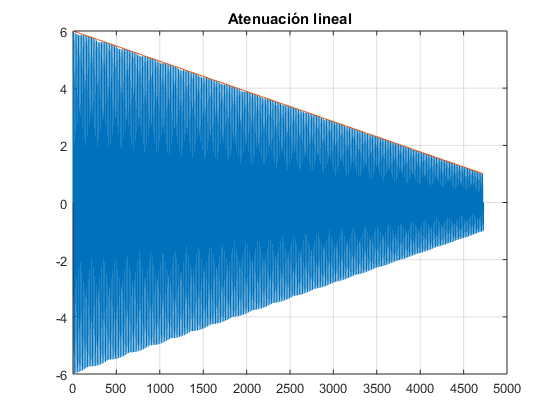
\includegraphics[width=\textwidth]{Lin_Ate.png}
		\caption{Senoidal de 50 Hz con atenuación lineal}
		\label{Figura: LinAte}
	\end{subfigure}
	\hfill
	\begin{subfigure}[htbp]{0.4\textwidth}
		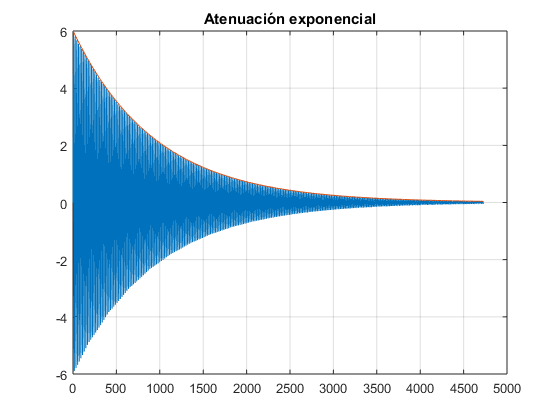
\includegraphics[width=\textwidth]{Exp_Ate.png}
		\caption{Senoidal de 50 Hz con atenuación exponencial}
		\label{Figura: ExpAte}
	\end{subfigure}
	\hfill
	\begin{subfigure}[htbp]{0.4\textwidth}
		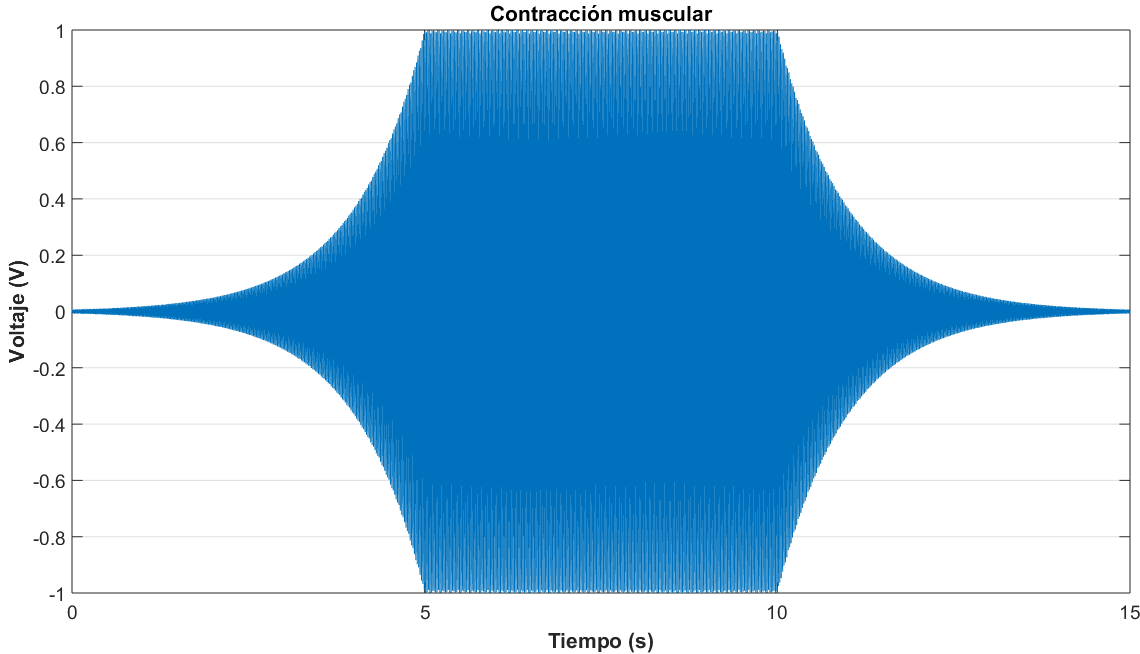
\includegraphics[width=\textwidth]{Contra.png}
		\caption{Senoidal de 50 Hz simulando una contracción muscular}
		\label{Figura: Contra}
	\end{subfigure}	
	\caption{Señales creadas para la evaluación del protocolo de comunicación}
	\label{Figura: SenalesEva}
\end{figure}

\section{Procesamiento de sEMG}
Relacionado al procesamiento de sEMG se han diseñado filtros pasa altas Butterworth con frecuencia de corte de 3 Hz para retirar el offset que suele presentar la señal de sEMG, pero aún no se ha tomado la decisión sobre qué banda trabajar para obtener información útil del sEMG para control.

En cuanto a los descriptores de amplitud ya se implementaron en Simulink tanto el RMS como el ARV, y por el momento ha dado mejores resulado el RMS.

\section{Mapeo sEMG-FES}
Utilizando el descriptor RMS se realizó una prueba para observar si el sistema decodificador y algún descriptor de amplitud eran compatibles con el bloque del RehaStim. Dicha prueba consistió en conectar el bloque del estimulador al resto del sistema diseñado y observar que entraran bien los datos al estimulador. Para ir variando el valor del RMS simplemente se tomó una senoidal y se fue variando su amplitud. El sistema obtenido tras esta prueba se muestra en la Figura \ref{Figura: Read2Stim}.

\begin{figure}[htbp]
	\centering
	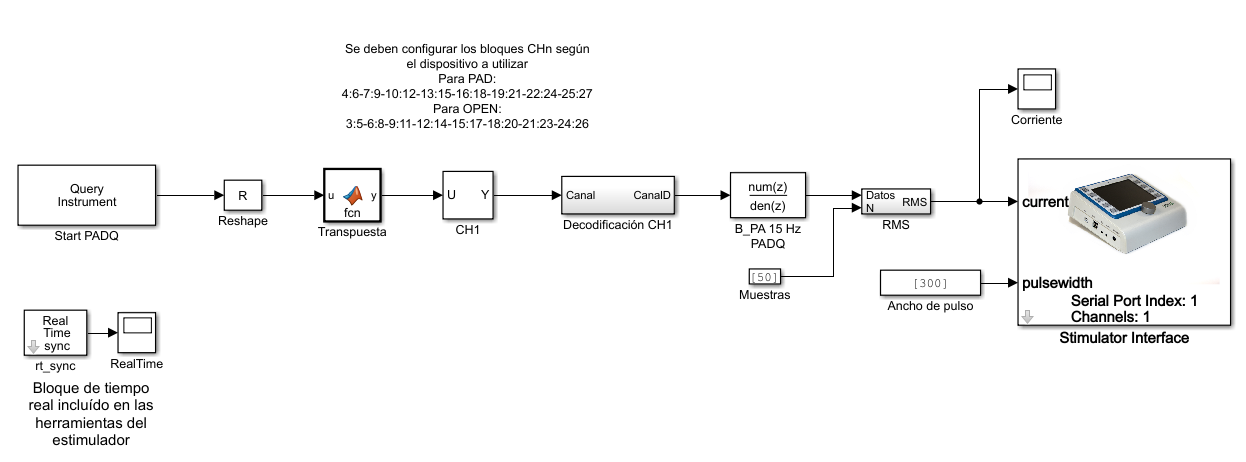
\includegraphics[width=\textwidth]{Read2Stim.png}
	\caption{Sistema utilizado para realizar prueba de compatibilidad entre el bloque decodificador y el bloque RehaStim}
	\label{Figura: Read2Stim}
\end{figure}